\section{Resultados} \label{sec:result}

Neste capítulo é mostrado um breve resultado do que foi realizado até agora.


\subsection{Planejamento do Problema} \label{subsec:planexp}

Assim como foi mostrado na seção \ref{subsubsec:etp} os passos da dissertação com que cada modelo e os métodos que podem ser usados para responder às perguntas de pesquisa abordadas na seção \ref{subsubsec:obespec}. Com os passos podem dar uma cronologia lógica do que foi adquirido ao longo do tempo com os dados SANEPAR.


\subsubsection{An\'alise Explorat\'oria dos dados (EDA)}

A partir do passo \ref{etp:1}, foi realizado o EDA (Exploratory Data Analysis) para processar os dados obtidos até o momento. O EDA permite responder às questões de pesquisa levantadas. Conforme mencionado por \citeonline{Yu2016}, na era dos grandes dados, é desafiador descobrir as regras, modelos analíticos e hipóteses por trás dos volumes massivos de dados caóticos, não estruturados e multimídia coletados por meio de vários canais. A análise exploratória de dados foi promovida por John Tukey como uma abordagem para explorar os dados, resumir suas principais características e formular hipóteses que possam direcionar a coleta adicional de dados e experimentos. No contexto de grandes análises de dados, várias técnicas de EDA têm sido adotadas.

Ao analisar a pergunta \ref{q1}, que relaciona a demanda com a variável prevista e a pressão para a variável PT01, pode-se observar na Figura \ref{fig:person} que ambas as variáveis apresentam uma correlação quase perfeita, com um coeficiente de correlação de Pearson ($r$) igual a 1. Portanto, para responder a essa pergunta, basta observar a correlação de Pearson na Figura \ref{fig:person}.

Para responder à pergunta \ref{q2}, é criada uma tabela para fornecer uma resposta mais completa.


\begin{table}[!htb]
	\centering
	\caption{Descrição estatística dos dados com o filtro aplicado das 18h às 21h}\label{tb:est}
	\begin{tabular}{@{}cccccccccc@{}}
		\toprule
		\textbf{18 a 21h}  & \textbf{B1} & \textbf{B2} & \textbf{B3} & \textbf{LT01} & \textbf{FT01} & \textbf{FT02} & \textbf{FT03} & \textbf{PT01} & \textbf{PT02} \\ \midrule
		\textbf{Contagem} & 4385    & 4385     & 4385     & 4385      & 4385       & 4385       & 4385       & 4385       & 4385       \\
		\textbf{Média}      & 51,94       & 27,81       & 6,41        & 3,24          & 112,68        & 132,93        & 112,41        & 4,11          & 20,80         \\
		\textbf{STD}       & 17,14       & 17,61       & 16,77       & 0,70          & 132,59        & 44,78         & 31,33         & 0,76          & 6,14          \\
		\textbf{Min}       & 0           & 0           & 0           & 0,29          & 0             & 0             & 0             & 0,88          & 0             \\
		\textbf{25\%}      & 57,84       & 0           & 0           & 2,79          & 0,12          & 123,96        & 111,66        & 3,62          & 21,72         \\
		\textbf{50\%}      & 57,99       & 34,91       & 0           & 3,30          & 0,12          & 136,00        & 118,82        & 4,15          & 22,05         \\
		\textbf{75\%}      & 57,99       & 38,02       & 0           & 3,78          & 264,27        & 148,20        & 125,63        & 4,66          & 23,02         \\
		\textbf{Max}       & 59,99       & 59,99       & 59,99       & 4,40          & 383,87        & 326,17        & 194,35        & 5,68          & 28,08         \\ \bottomrule
	\end{tabular}
	
	\fonte{Elaboração própria a partir de dados da SANEPAR (2018 a 2020)}
\end{table}



Na Tabela \ref{tb:est}, o desvio padrão é representado pela sigla STD, que corresponde à expressão em inglês ``\textit{standard deviation}''. Além disso, em resposta à pergunta \ref{q2}, é importante mencionar que, assim como em qualquer empresa de tratamento de água, é utilizado um mecanismo de acionamento automático chamado "trava de segurança" para evitar que o nível do tanque chegue a zero e haja falta de água nos locais abastecidos por esse tanque. O nível mínimo que o tanque pode alcançar é de $5.29 m^3$ (equivalente a 5,29 litros). As bombas são ativadas em sua potência máxima para evitar que sejam acionadas quando o nível do tanque. No entanto, a bomba 1 ainda estaria operando para completar o nível do tanque caso ele esteja dentro dessa faixa.

Em situações de demanda de pico, uma abordagem ideal, embora não necessariamente a mais econômica, seria ter um tanque de reserva adicional e instalar uma tubulação que os conecte. Durante o dia, ambos os tanques seriam abastecidos e, à noite, por meio da ação da gravidade, eles manteriam o mesmo nível até que o consumo atinja um ponto em que as bombas sejam acionadas. Essa estratégia permite um abastecimento contínuo e eficiente de água.


Na pergunta \ref{q3}, observa-se que o tanque tem uma capacidade máxima de $4,256 m^3$, o que equivale a $4.256$ litros. Para atender a essa demanda e manter o tanque quase cheio ou sempre cheio, é necessário que o fluxo de entrada esteja na faixa de $[238, 302] \ m^3/h$, o fluxo de gravidade esteja entre $[126, 182] \ m^3/h$, o fluxo de retorno esteja entre $[110, 144] \ m^3/h$, a pressão de sucção esteja entre $[1.92, 4.24] \ mca$ e a pressão de retorno esteja entre $[21, 24] \ mca$.

Para responder à pergunta \ref{q4}, o ponto de equilíbrio, onde as bombas não precisam ser acionadas, ocorre quando o fluxo de FT01 é de $211 \ m^3/h$, FT02 é de $114 \ m^3/h$, FT03 é de $100 \ m^3/h$ e o nível do tanque está em $3.545 \ m^3$.
No que diz respeito à pergunta \ref{q5}\ref{q5:a}, o nível do tanque deve ser de $4,00 \ m^3$ para evitar o funcionamento das bombas durante as horas de pico.

\subsubsection{M\'ultiplas entradas e sa\'ida \'unica (MISO)}

Nesta \ref{etp:2} os modelos que foram mais cobertos no decorrer da dissertação são os modelos ARIMA ou aqueles derivados deste modelo e os modelos regressivos fora do LR têm múltiplas entradas e uma saída da variável que se prevê a LT01, as outras variáveis servem como suporte para melhorar os modelos do tipo ARX ou modelos com variáveis exógenas. Os modelos ARIMA sem a variável exógena são apenas uma entrada semelhante com LR.

\subsubsection{Decomposi\c c\~ao STL}\label{subsubsec:stl}

A decomposição sazonal e de tendência utilizando o procedimento de Loess (STL) é uma técnica amplamente utilizada para decompor séries temporais em seus componentes sazonais, de tendência e restantes. De acordo com \citeonline{Theodosiou20111178}, o método STL realiza a decomposição aditiva dos dados por meio de uma sequência de aplicações do Loess mais suave, onde regressões polinomiais ponderadas localmente são aplicadas em cada ponto do conjunto de dados, tendo como variáveis explicativas os valores mais próximos do ponto cuja resposta está sendo estimada.

A decomposição STL é especialmente útil para identificar e isolar padrões sazonais e de tendência presentes nas séries temporais. Ela permite a separação dos componentes sazonais, que ocorrem em intervalos regulares ao longo do tempo, da componente de tendência, que indica a direção geral dos dados ao longo do tempo. A decomposição também resulta em uma componente restante, que representa a variação não explicada pelos componentes sazonais e de tendência.

Ao aplicar a decomposição STL, a série temporal pode ser expressa como a soma dos componentes sazonais, de tendência e restantes. Essa técnica é útil para análise e modelagem de séries temporais, pois proporciona uma compreensão mais clara dos padrões de variação presentes nos dados.

A decomposição STL é formalmente definida como:

\begin{eqnarray}
	y_t=f\left(S_t, T_t, R_t\right)&=&\left\{\begin{array}{l}
		y_t=S_t+T_t+R_t \quad \text { aditivo } \\
		y_t=S_t T_t R_t \quad \text { multiplicativo }
	\end{array}\right. \label{eq:stl}
\end{eqnarray}

\begin{figure}[!htb]
	\centering
	\caption{Decomposição STL}
	\begin{subfigure}{1\textwidth}
		\includegraphics[width=\linewidth]{"Resultados/Figuras/STL aditiva"}
		\caption{Decomposição STL aditiva dos dados coletados}
		\label{fig:stl-aditiva}
	\end{subfigure}
		
	\begin{subfigure}{1\textwidth}
		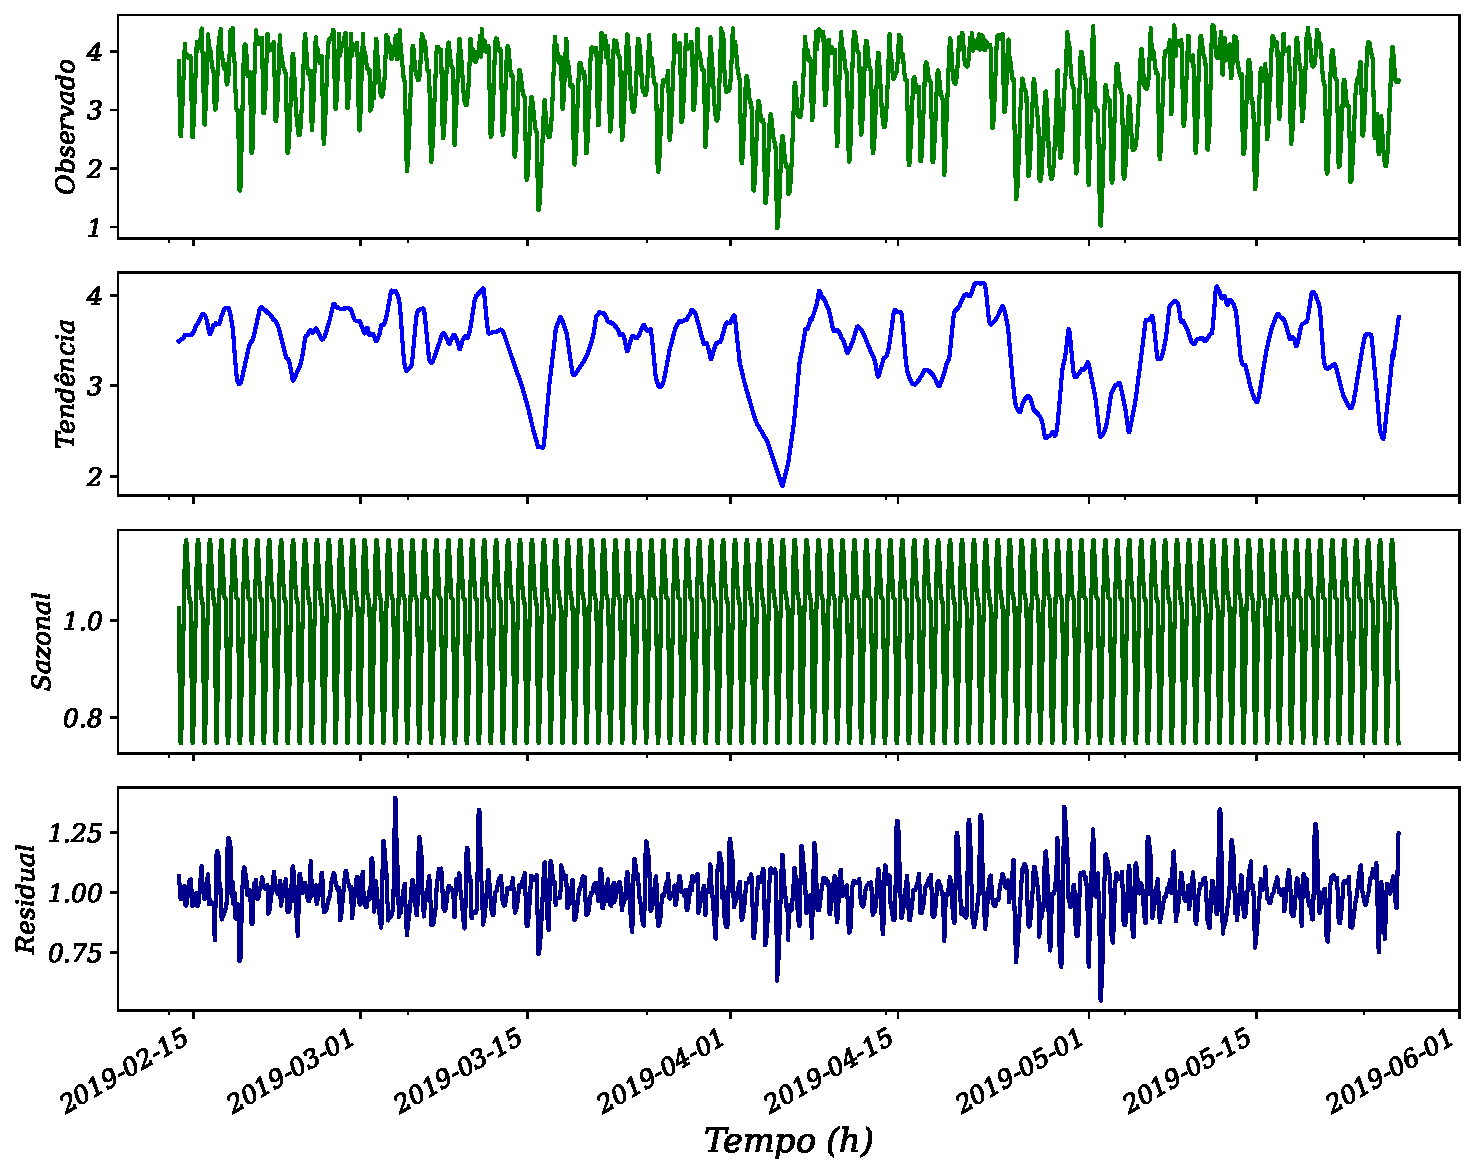
\includegraphics[width=\linewidth]{Resultados/Figuras/STL}
		\caption{Decomposição STL multiplicativa dos dados coletados}
		\label{fig:stl}
	\end{subfigure}
	
	\fonte{Elaboração própria a partir de dados da SANEPAR (2018 a 2020)}
\end{figure}

Na resposta à pergunta \ref{q5}\ref{q5:b}, as Figuras \ref{fig:stl-aditiva} e \ref{fig:stl} fornecem informações sobre a presença de tendência, sazonalidade e resíduos na série temporal.

Através da decomposição, é possível analisar se a série apresenta tendência, sazonalidade e resíduos. Ao observar as Figuras \ref{fig:stl-aditiva} e \ref{fig:stl}, é evidente que os dados exibem ambos os padrões. Isso indica que a série é estacionária, como confirmado pelo seguinte teste.

Teste de Dickey-Fuller (DF) Aumentado:
\begin{itemize}
	\item Estatística de teste ADF: $-4,25$
	\item Valor de p: $0,001$
	\item Atrasos utilizados: $21$
	\item Observações: $1074$
	\item Valor crítico ($1\%$): $-3,44$
	\item Valor crítico ($5\%$): $-2,86$
	\item Valor crítico ($10\%$): $-2,57$
\end{itemize}

Com base na forte evidência contra a hipótese nula, podemos rejeitar a hipótese nula. Isso indica que os dados não possuem raiz unitária e são estacionários em \ref{q5}\ref{q5:c}. Identificar as horas de pico entre 18h e 21h não é uma tarefa fácil. No entanto, ao observar a Figura \ref{fig:hist}, podemos notar um aumento na demanda durante essas horas durante o ano de 2020.
	
	
	\begin{figure}[!htb]
		\centering
		\caption{Violino no nível do reservatório}
		\label{fig:hist}
		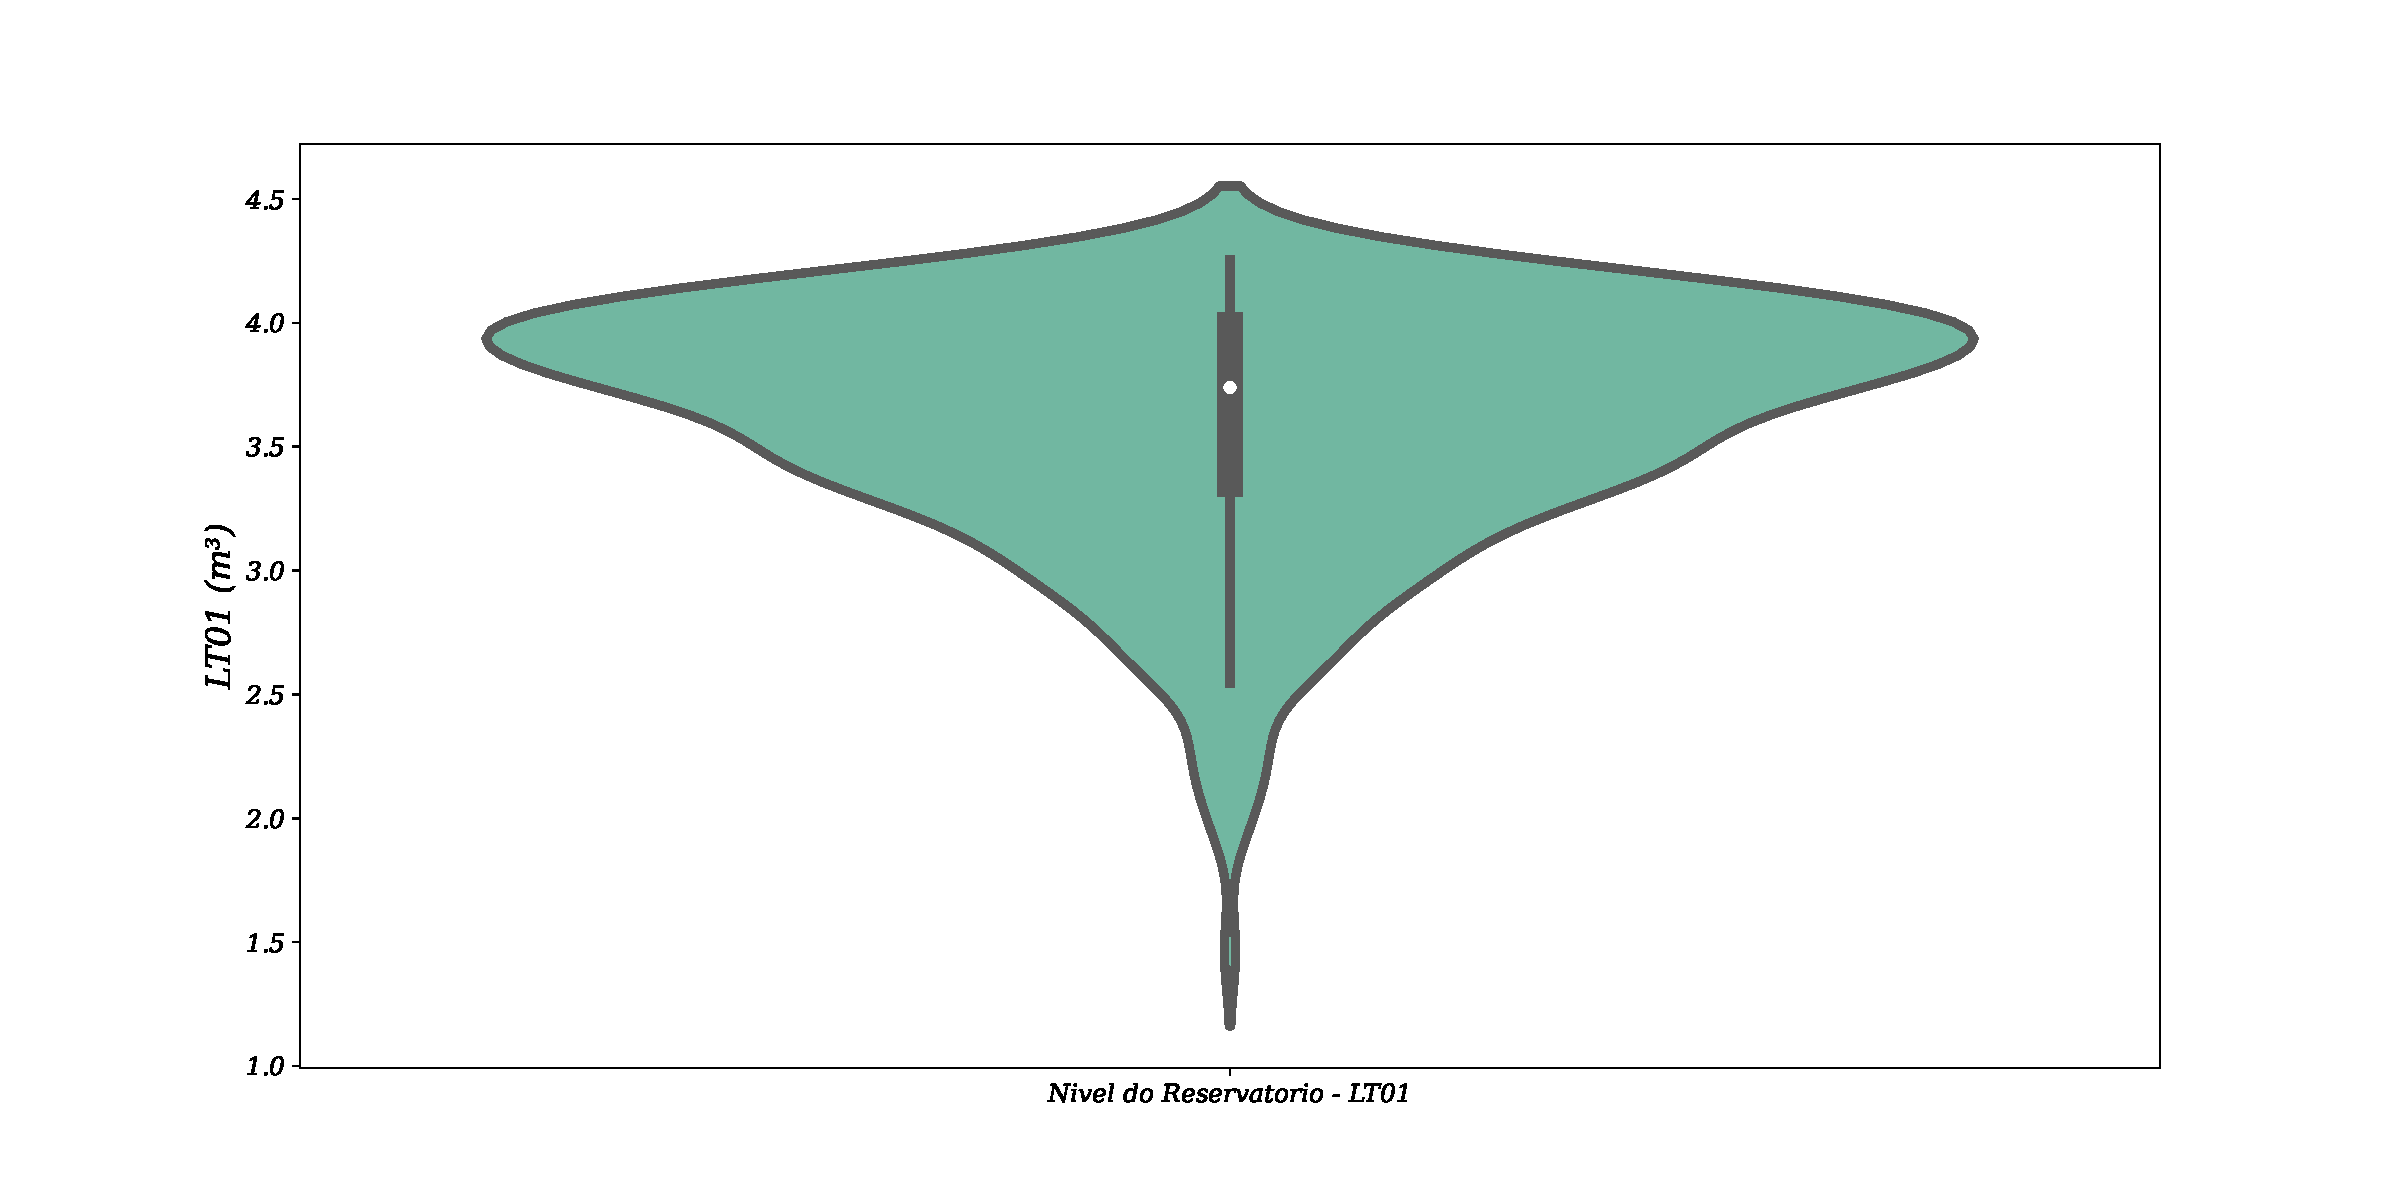
\includegraphics[width=0.9\linewidth]{Resultados/Figuras/viol}
		
		\fonte{Elaboração própria a partir de dados da SANEPAR (2018 a 2020)}
	\end{figure}
	
Conforme mencionado na subseção \ref{subsubsec:motivacao}, as anomalias climáticas ocorridas em 2020, especialmente a falta de chuvas, tiveram um impacto significativo nos resultados. Isso contribuiu para as mudanças observadas na demanda de água ao longo desse período.

Com relação à pergunta \ref{q5}\ref{q5:d}, durante as horas de pico, é necessário que o nível do tanque esteja dentro da faixa de $[3.545,4.256] m^3$ para evitar o acionamento das bombas. Manter o nível do tanque dentro dessa faixa permitirá que o sistema opere de forma eficiente, atendendo à demanda sem a necessidade de acionar as bombas.
	
	
	\begin{figure}[!htb]
		\centering
		\caption{Violino da vazão de recalque}
		\label{fig:ft03}
		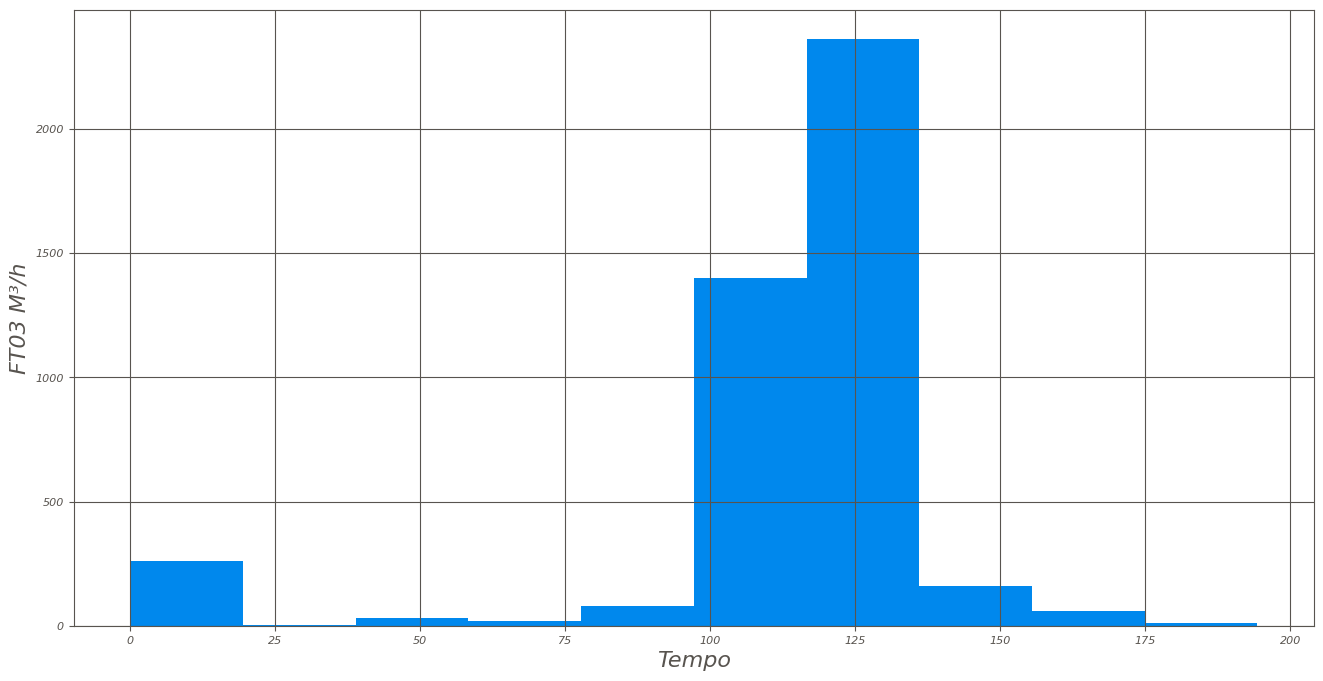
\includegraphics[width=0.9\linewidth]{Resultados/Figuras/ft03}
		
		\fonte{Elaboração própria a partir de dados da SANEPAR (2018 a 2020)}
	\end{figure}
	
Para responder à pergunta \ref{q5}\ref{q5:e}, a Figura \ref{fig:ft03} ilustra como a vazão pode ser afetada pelo nível do tanque. É interessante observar que a vazão de recalque tem um impacto mais significativo no nível do tanque em comparação com as outras vazões. Isso ocorre porque a vazão de recalque está associada à injeção de água diretamente no tanque por meio da bomba localizada próxima à base do tanque. Por outro lado, as demais vazões apresentam alguns valores ausentes, o que limita sua influência na análise geral.	
	


De acordo com o \citeonline{Reisen2017115}, o teste DF tem as seguintes equações

\begin{eqnarray}
	z_t&=& y_t+\theta \beta_t, \qquad t=1,\ldots, T, \label{eq:df3}\\	
	\hat{\rho}_{\mathrm{DF}}-1&=&\frac{\sum_{t=1}^T z_{t-1} \Delta z_t}{\sum_{t=1}^T z_{t-1}^2} \label{eq:regdf}
\end{eqnarray}

De \eqref{eq:regdf} onde $\Delta z_t=z_t-z_{t-1}$. Sob a hipótese nula $\left(H_0\right)$ : `` $\rho=1$'', as estatísticas do teste DF e suas distribuições limitantes são dadas da seguinte forma:


\begin{eqnarray}
	T\left(\hat{\rho}_{\mathrm{DF}}-1\right)=T \frac{\sum_{t=1}^T z_{t-1} \Delta z_t}{\sum_{t=1}^T z_{t-1}^2}
\end{eqnarray}
e


\begin{eqnarray}
	\hat{\tau}_{\mathrm{DF}}&=&\frac{\hat{\rho}_{\mathrm{DF}}-1}{\hat{\sigma}_{\mathrm{DF}}\left(\sum_{t=1}^T z_{t-1}^2\right)^{-1 / 2}} \label{eq:df}
\end{eqnarray}

De \eqref{eq:df} onde $\hat{\sigma}_{\mathrm{DF}}^2=T^{-1} \sum_{t=1}^T\left(\Delta z_t-\left(\hat{\rho}_{\mathrm{DF}}-1\right) z_{t-1}\right)^2 .$



Suponha que $\left(z_t\right)_{1 \leq t \leq T}$ são dadas por \eqref{eq:df3}, então quando $\rho=1$,


\begin{eqnarray}
	T\left(\hat{\rho}_{\mathrm{DF}}-1\right) \stackrel{d}{\longrightarrow} \frac{W(1)^2-1}{2 \int_0^1 W(r)^2 \mathrm{~d} r}-\left(\frac{\theta}{\sigma}\right)^2 \frac{\pi}{\int_0^1 W(r)^2 \mathrm{~d} r}, \text { como } T \rightarrow \infty \\
	\hat{\tau}_{\mathrm{DF}} \stackrel{d}{\longrightarrow}\left[1+2(\theta / \sigma)^2 \pi\right]^{-1 / 2}\left\{\frac{W(1)^2-1}{2\left(\int_0^1 W(r)^2 \mathrm{~d} r\right)^{1 / 2}}-\frac{(\theta / \sigma)^2 \pi}{\left(\int_0^1 W(r)^2 \mathrm{~d} r\right)^{1 / 2}}\right\} \\
	\quad \operatorname{como} T \rightarrow \infty\label{eq:df2}
\end{eqnarray}

A partir de \eqref{eq:df2}, onde $\stackrel{d}{\longrightarrow}$ denota convergência na distribuição e onde $\left\{W(r), r \in[0,1]\right\}$ denota o movimento Browniano padrão.

O ACF (do inglês \textit{Auto-Correlation Function}) é uma medida estatística utilizada para identificar a presença de correlação serial em uma série temporal. Ele calcula a autocorrelação entre os valores da série em diferentes defasagens, ou seja, a correlação entre os valores atuais e os valores passados da série. 

O ACF é útil para analisar a dependência temporal dos dados e identificar padrões de sazonalidade, tendência ou outros efeitos temporais. Através do ACF, é possível avaliar se a série exibe autocorrelação significativa em defasagens específicas, o que pode indicar a presença de não estacionariedade ou estrutura temporal que precisa ser considerada na análise ou modelagem da série temporal.

\begin{figure}[!htb]
	\centering
	\caption{Autocorrelação e Autocorrelação parcial}
	\label{fig:acf}
	
	
	\begin{subfigure}{0.9\textwidth}
		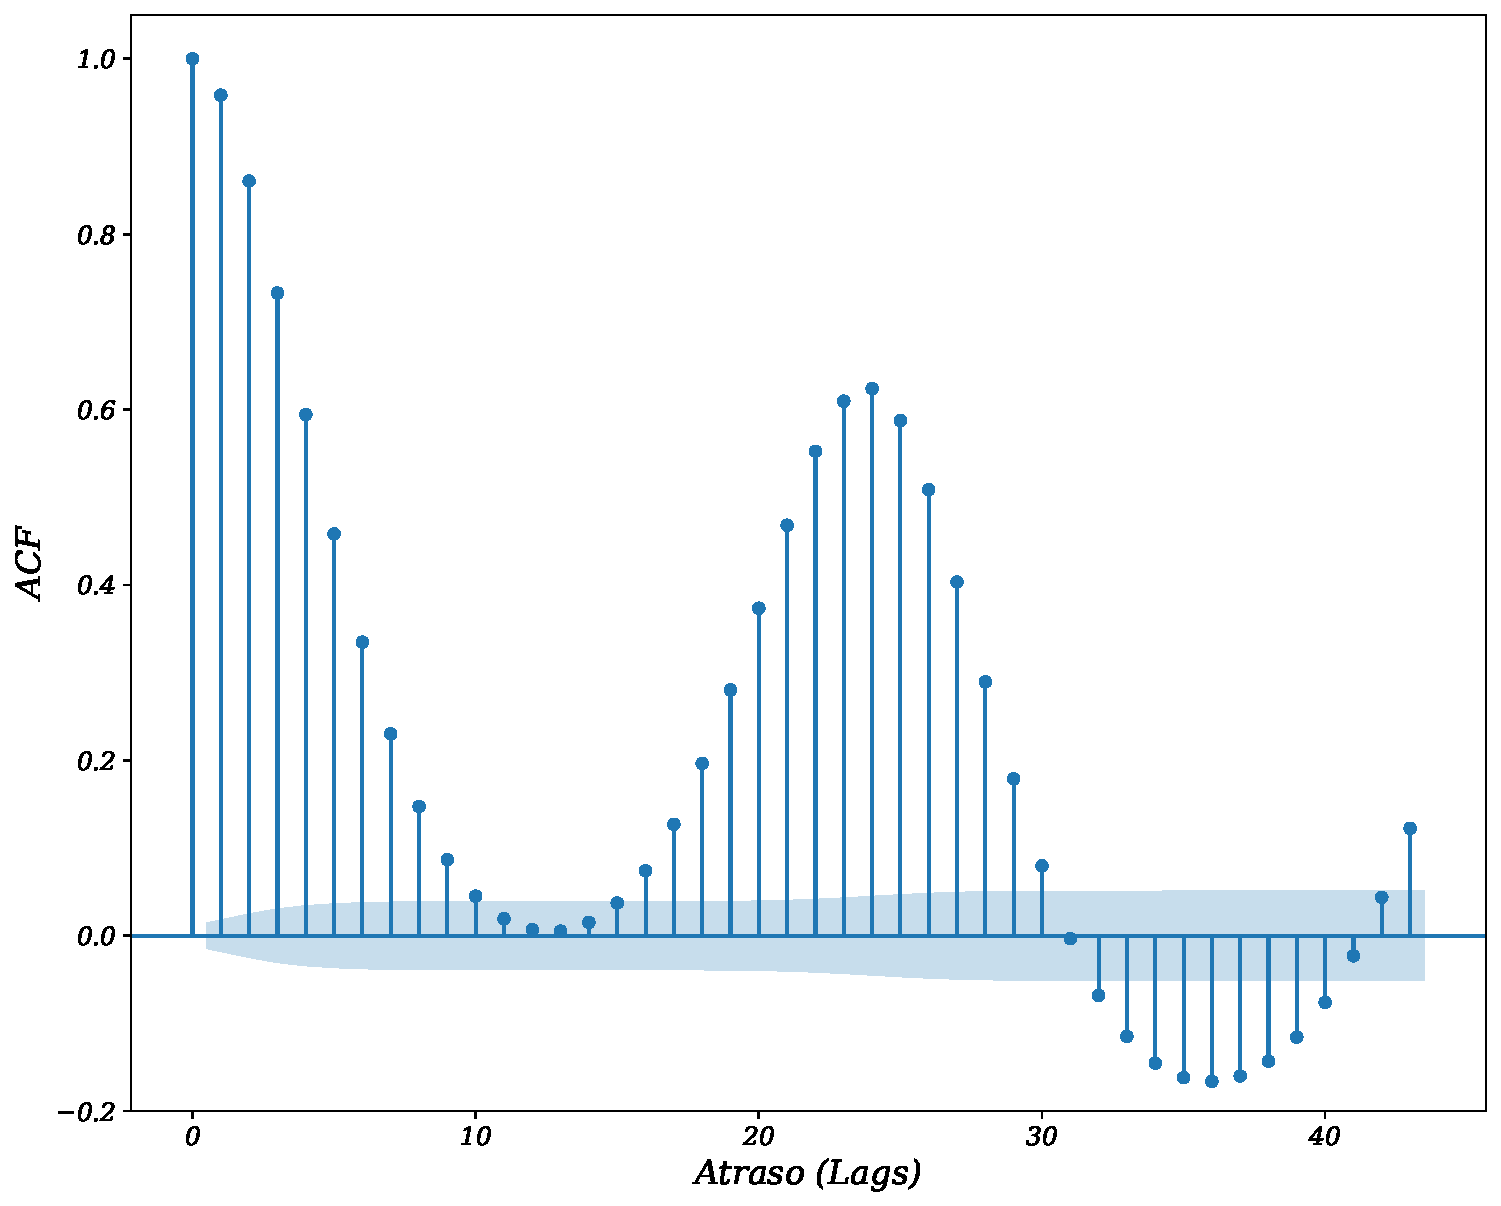
\includegraphics[width=\linewidth]{Resultados/Figuras/acf} 
		\caption{ACF}\label{fig:acfa}
	\end{subfigure}
	

	\begin{subfigure}{0.9\textwidth}
		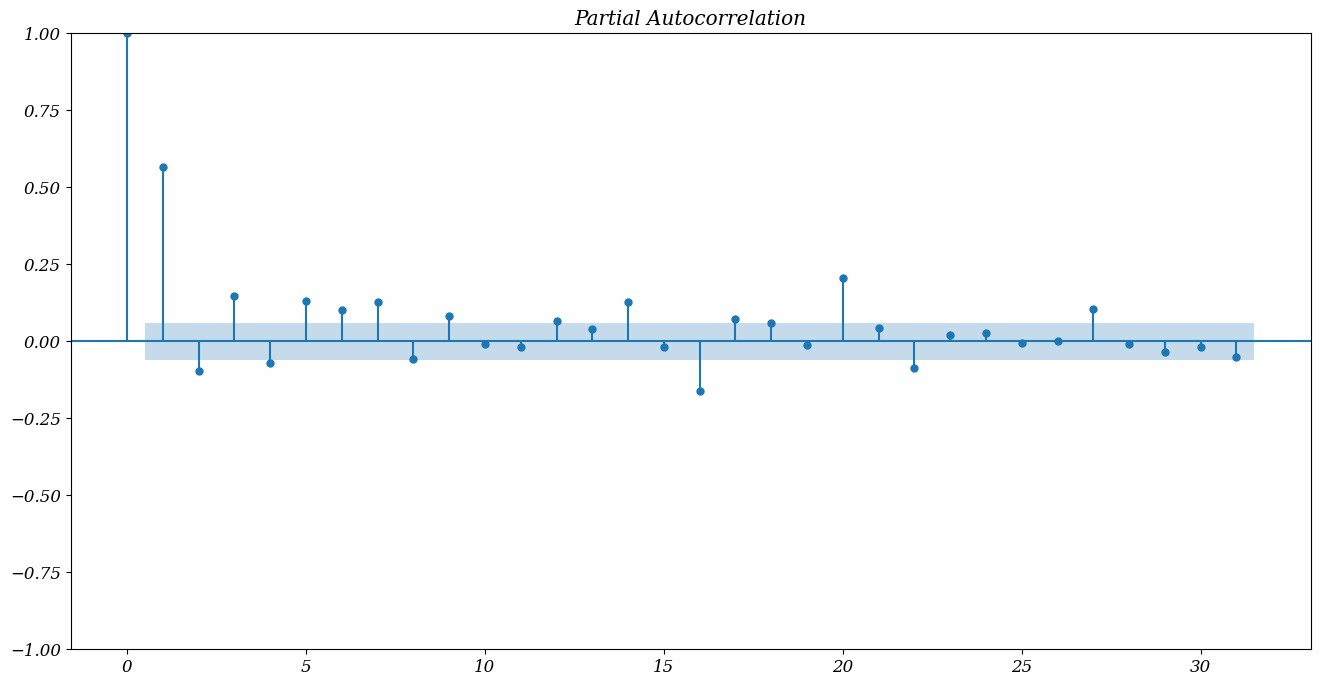
\includegraphics[width=\linewidth]{Resultados/Figuras/pacf}
		\caption{PACF}\label{fig:pacf}
	\end{subfigure}
	
	\fonte{Elaboração própria a partir de dados da SANEPAR (2018 a 2020)}
\end{figure}

A estatística ADF (do ingê \textit{Augmented Dickey-Fuller}) de $-4,27$ indica a evidência de estacionariedade na série temporal. Quanto mais negativo for o valor da estatística ADF, maior é a evidência de estacionariedade nos dados.

O valor-p de $0,0005$, por sua vez, está associado ao teste ADF. O valor-p é uma medida estatística que representa a probabilidade de obter um resultado igual ou mais extremo do que o observado, sob a suposição de que a hipótese nula seja verdadeira. No caso do teste ADF, a hipótese nula é a presença de raiz unitária na série temporal, o que indica não estacionariedade. Assim, um valor-p baixo (geralmente abaixo de um nível de significância predefinido, como 0,05) sugere que a série temporal é estacionária, enquanto um valor-p alto sugere que a série temporal é não estacionária. Neste caso, o valor-p de $0,0005$ é bastante baixo, o que indica forte evidência contra a hipótese nula e sugere que a série temporal é estacionária.

Na Figura \ref{fig:acf}, pode-se observar a diferença entre a autocorrelação (ACF) exibida na Figura \ref{fig:acfa} e a autocorrelação parcial (PACF) exibida na Figura \ref{fig:pacf}. A autocorrelação é uma medida da correlação entre os valores da série temporal em diferentes defasagens, levando em consideração tanto a correlação direta quanto a correlação indireta. Por outro lado, a autocorrelação parcial mede apenas a correlação direta entre os valores, desconsiderando a influência das defasagens intermediárias. Essas análises são úteis para identificar padrões e relações de dependência entre os valores da série temporal, fornecendo informações importantes para a modelagem e previsão desses dados.

O intervalo de confiança padrão de 95\% é representado pela marca azul na Figura. As observações que estão fora desse intervalo são consideradas estatisticamente correlacionadas, indicando a presença de padrões ou estrutura na série temporal.

A correlação visualizada na Figura \ref{fig:acf} é fundamental para a interpretação do teste DF. Em uma série de ruído branco, os valores são completamente aleatórios e não apresentam correlação significativa. Portanto, quando há correlação presente na série, isso indica a existência de padrões ou dependências entre os valores, o que pode ser explorado para a modelagem e previsão da série temporal.

\begin{figure}[!htb]
	\centering
	\caption{Ruído branco}
	\label{fig:ruido-branco}
	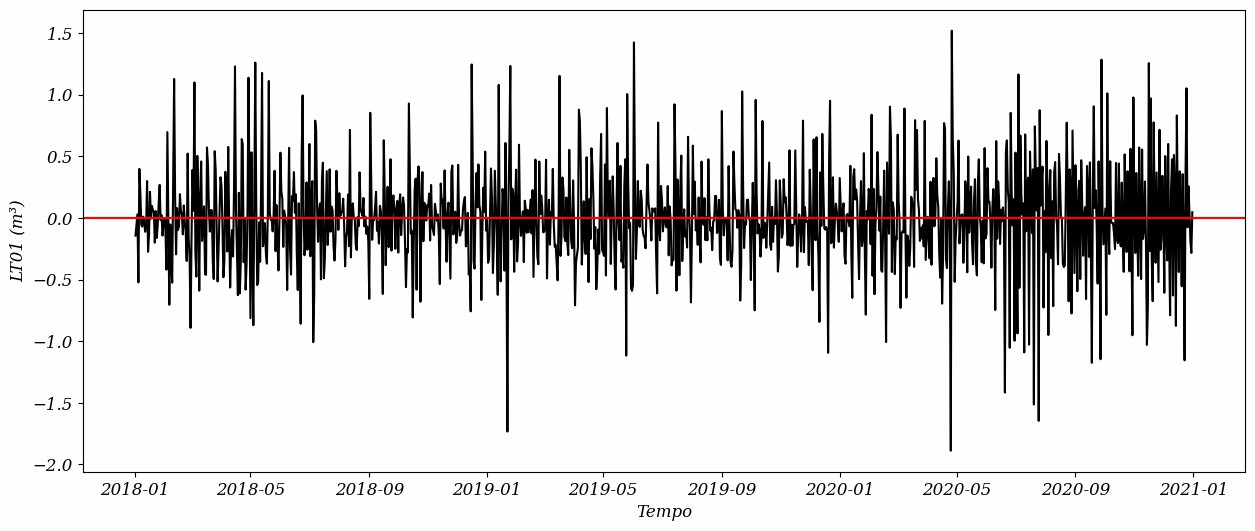
\includegraphics[width=0.9\linewidth]{Resultados/Figuras/ruido-branco}
	
	\fonte{Elaboração própria a partir de dados da SANEPAR (2018 a 2020)}
\end{figure}

Na Figura \ref{fig:ruido-branco}, é possível observar uma série temporal que pode ser caracterizada como ruído branco. Uma série temporal é considerada ruído branco se suas variáveis forem independentes e distribuídas de forma idêntica, com média zero. Isso implica que todas as variáveis possuem a mesma variância ($\sigma^2$) e que cada valor não possui correlação com os demais valores da série.

Além disso, é importante destacar o comprimento dos zeros na variável prevista, o que conclui a etapa \ref{etp:3}.

\subsubsection{Separa\c c\~ao dos dados}\label{subsubsec:divisao}

Na etapa \ref{etp:4}, os dados foram divididos em conjuntos de treinamento, teste e validação. Essa prática é comum entre profissionais de aprendizado de máquina, pois permite avaliar o desempenho do modelo em conjuntos de dados diferentes.

Em relação ao processamento de modelos de aprendizado profundo, é importante mencionar as inovações trazidas pela empresa Nvidia ao longo dos anos, especialmente no campo do processamento de imagens. O lançamento da placa de vídeo GeForce RTX 4090 tem sido bastante aguardado tanto por gamers quanto por profissionais que lidam com aprendizado de máquina.

No contexto do estudo, foram utilizados dois computadores para realizar os cálculos dos modelos. Um deles é equipado com um processador Intel Core i5-3330 e o outro é um notebook com um processador Intel Core i7-5500. Ambos os processadores possuem 4 threads, sendo que o notebook possui 2 núcleos físicos e o i5 possui 4 núcleos físicos. Cada processador tem suas especificações e desempenho adequados a diferentes necessidades. Vale ressaltar que não é obrigatório utilizar as últimas gerações de processadores para realizar esses processamentos, e sim compreender e aplicar corretamente os recursos disponíveis.

Quanto à divisão dos dados, foi adotada uma estratégia básica em que 70\% dos dados foram destinados ao conjunto de treinamento e os 30\% restantes foram reservados para o conjunto de teste. Dentro dos 70\% de treinamento, foi realizada uma subdivisão em que 80\% desses dados foram usados novamente para treinamento e os 20\% restantes foram utilizados para validação. Essa abordagem foi implementada em linguagem de programação para facilitar o processo e evitar a necessidade de recalculá-la a cada modificação do modelo.

\subsubsection{Estrat\'egia de Previs\~ao}\label{subsubsec:est}

A estratégia recursiva é mencionada por \citeonline{PETROPOULOS2022705} como uma abordagem eficaz na previsão de séries temporais de múltiplos passos. De acordo com o autor, essa estratégia envolve o uso de previsões anteriores como entradas para prever os próximos passos da série temporal. A abordagem recursiva tem demonstrado potencial para melhorar a acurácia das previsões de séries temporais de longo prazo.

Na Etapa \ref{etp:5}, discute-se a previsão dos dados em uma janela de horizonte de previsão estendida, abrangendo diferentes períodos de tempo, como um dia, uma semana, duas semanas e um mês. Essa estratégia de previsão recorrente permite a comparação entre modelos de regressão e modelos ARIMA em diferentes horizontes temporais.

Essa abordagem é vantajosa, pois cada modelo possui suas próprias características e desempenho ao lidar com previsões de curto prazo, como um dia, e previsões de prazo mais longo, como um mês. Ao utilizar uma janela de previsão mais ampla, é possível observar e avaliar melhor as diferenças entre os modelos e analisar seu desempenho em horizontes de tempo variados.

\textbf{Validação e ajuste do modelo}
na etapa \ref{etp:6}, o horizonte de previsão foi personalizado com base no método recursivo de previsão de série temporal e na previsão do nível do tanque LT01. Foram selecionados os seguintes passos para a previsão à frente: uma hora, seis horas, doze horas e um dia. Essa escolha do horizonte de previsão foi feita levando em consideração a estratégia recursiva e os objetivos específicos do estudo. Identifica-se que essa janela de tempo proporciona uma análise mais adequada e comparável entre os modelos utilizados.

Foram utilizados os parâmetros obtidos pelo autoARIMA, que são $(p = 7, d = 0, q = 0) (P = 2, D = 1, Q = 1)_{M = 12}$, mas foram ajustados para obter um melhor resultado, sendo $(p = 7, d = 1, q = 7) (P = 2, D = 1, Q = 1)_{M = 12}$. Na Tabela \ref{tab:autoarima_params}, são exibidos todos os modelos obtidos por esse método do ``autoARIMA'' e ajustados para que obtenham o melhor resultado.
\(p\): Ordem do componente AR (\textit{Auto-Regressivo}),
\(d\): Número de diferenciações não sazonais,
\(q\): Ordem do componente MA (\textit{Média Móvel}),
\(P\): Ordem do componente AR sazonal,
\(D\): Número de diferenciações sazonais,
\(Q\): Ordem do componente MA sazonal,
\(M\): Período sazonal (número de observações em um ciclo sazonal).
Na Tabela \ref{tb:resltsar} mostra como a biblioteca do Python autoARIMA obteve os resultados dos parâmetros, exibindo o STD e os intervalos de confiança nos quais o modelo alcançou o melhor desempenho. O leve ajuste realizado não altera significativamente os parâmetros obtidos nesta biblioteca, permitindo que cada modelo seja trabalhado de maneira eficiente.

\begin{table}[!htb]
	\centering
	\caption{Parâmetros utilizados nos modelos ARIMA e seus antecessores obtidos pelo ``autoARIMA'' do Python.}
	\label{tab:autoarima_params}
	\small
	\begin{tabular}{
			>{\centering\arraybackslash}p{5.5cm}
			>{\centering\arraybackslash}p{6cm}
			>{\centering\arraybackslash}p{3cm}
		}
		\toprule
		\textbf{Modelo} & \textbf{Parâmetros Utilizados} & \textbf{Método de Estimação} \\
		\midrule
		AR(p) & \( p = 7 \) & AutoARIMA \\
		ARX(p) & \( p = 7 \) & AutoARIMA \\
		MA(q) & \( q = 7 \) & AutoARIMA  \\
		ARMA(p, q) & \( p = 7 \), \( q = 7 \) & AutoARIMA  \\
		ARIMA(p, d, q) & \( p = 7 \), \( d = 1 \), \( q = 7 \) & AutoARIMA  \\
		ARIMAX(p, d, q) & \( p = 7 \), \( d = 1 \), \( q = 7 \) & AutoARIMA  \\
		SARIMA(p, d, q)(P, D, Q) & \( p = 7 \), \( d = 1 \), \( q = 7 \), \( P = 2 \), \( D = 1 \), \( Q = 1 \), \( M = 12 \) & AutoARIMA  \\
		SARIMAX(p, d, q)(P, D, Q, M) & \( p = 7 \), \( d = 1 \), \( q = 7 \), \( P = 2 \), \( D = 1 \), \( Q = 1 \), \( M = 12 \) & AutoARIMA  \\
		\bottomrule
	\end{tabular}
\end{table}



\begin{table}[!htb]
	\centering
	\caption{SARIMAX$(7, 0, 0)\times(2, 1, [1], 12)$ Results} \label{tb:resltsar}
	\begin{tabular}{
			l
			S[table-format=1.4]
			S[table-format=1.4]
			S[table-format=3.3]
			S[table-format=1.3]
			S[table-format=1.3]
			S[table-format=1.3]
		}
		\toprule
		& {Coef} & {STD Err} & {z} & {P$>|z|$} & {[0,025} & {0,975]} \\
		\midrule
		Intercept & 0,0003 & 0,000 & 1,053 & 0,292 & -0,000 & 0,001 \\
		ar.L1 & 1,6149 & 0,011 & 141,865 & 0,000 & 1,593 & 1,637 \\
		ar.L2 & -0,8879 & 0,021 & -42,045 & 0,000 & -0,929 & -0,847 \\
		ar.L3 & 0,3167 & 0,024 & 13,033 & 0,000 & 0,269 & 0,364 \\
		ar.L4 & -0,1056 & 0,027 & -3,961 & 0,000 & -0,158 & -0,053 \\
		ar.L5 & -0,1099 & 0,028 & -3,928 & 0,000 & -0,165 & -0,055 \\
		ar.L6 & 0,1431 & 0,027 & 5,368 & 0,000 & 0,091 & 0,195 \\
		ar.L7 & -0,0673 & 0,015 & -4,583 & 0,000 & -0,096 & -0,039 \\
		ar.S.L12 & -0,1222 & 0,016 & -7,705 & 0,000 & -0,153 & -0,091 \\
		ar.S.L24 & 0,1692 & 0,014 & 12,244 & 0,000 & 0,142 & 0,196 \\
		ma.S.L12 & -0,8728 & 0,012 & -74,569 & 0,000 & -0,896 & -0,850 \\
		sigma2 & 0,0157 & 0,000 & 60,022 & 0,000 & 0,015 & 0,016 \\
		\bottomrule
	\end{tabular}
\end{table}


Para os modelos de gradiente \textit{boosting} e redes neurais artificiais, os hiperparâmetros foram otimizados usando a biblioteca Optuna do Python. Nesse contexto, são empregadas técnicas bayesianas, especificamente o algoritmo TPE, visando uma otimização mais eficiente.

Os modelos XGBoost e LightGBM tem como parâmetros e hiperparâmetros mostrado na Tabela \ref{tab:hiperparametros} a otimização dos paramétrios dos modelos XGBoost, LightGBM, RFR e DTR. Esses modelos, devido à sua semelhança, exibem tempos de desempenho próximos um do outro. 



\begin{table}[!htb]
	\centering
	\caption{Hiperparâmetros dos modelos}
	\label{tab:hiperparametros}
	\begin{tabular}{
			>{\centering\arraybackslash}p{2.2cm}
			>{\centering\arraybackslash}p{2.8cm}
			>{\centering\arraybackslash}p{1.9cm}
			>{\centering\arraybackslash}p{1.9cm}
			>{\centering\arraybackslash}p{1.9cm}
			>{\centering\arraybackslash}p{1.9cm}
			>{\centering\arraybackslash}p{1.9cm}
		}
		\toprule
		\textbf{Modelo} & \textbf{Estimadores} & \textbf{Profund. Máxima} & \textbf{Min. Amostras Divisão} & \textbf{Min. Amostras por Folha} & \textbf{Máx. Recursos} & \textbf{Taxa de Aprendizado} \\
		\midrule
		XGB Regressor & 503 & 5 & 7 & 2 & ``sqrt'' & 0,034 \\
		LGBM Regressor & 820 & 10 & 3 & 5 & ``auto'' & 0,014 \\
		Random Forest Regressor & 135 & 10 & 4 & 2 & None & N/A \\
		Decision Tree Regressor & N/A & 229 & 32 & 20 & None & N/A \\
		\bottomrule
	\end{tabular}
\end{table}



Os modelos de rede neural artificial, como RNN, ANN, CNN, GRU, LSTM e Transformer, obtidos na otimização do Optuna do Python, tiveram seus hiperparâmetros melhorados, conforme exibido na Tabela \ref{tab:hyperparameters_summary}. Esses modelos, por serem modelos de rede neural artificial, são melhores para otimizar do que os outros. 

\begin{table}[!htb]
	\centering
	\caption{Resumo dos Hiperparâmetros dos Modelos de Redes Neurais}
	\label{tab:hyperparameters_summary}
	\small
	\begin{tabular}{
			>{\centering\arraybackslash}p{1.8cm}
			>{\centering\arraybackslash}p{2cm}
			>{\centering\arraybackslash}p{2cm}
			>{\centering\arraybackslash}p{2cm}
			>{\centering\arraybackslash}p{2cm}
			>{\centering\arraybackslash}p{1.5cm}
			>{\centering\arraybackslash}p{2.5cm}
		}
		\toprule
		\textbf{Modelo} & \textbf{Unidades/ Layers} & \textbf{Heads/ Dimensões} & \textbf{Tamanho do Batch} & \textbf{Épocas} & \textbf{Dropout/ Learning Rate} & \textbf{Outros Parâmetros} \\
		\midrule
		LSTM & 128 & -- & 32 & 77 & -- & -- \\
		
		GRU & -- & -- & 32 & 50 & -- & -- \\
		
		Transformers & -- & 8 heads, 217; 433 & -- & 50 & -- & 2 camadas \\
		
		RNN & 79 & -- & 16 & 50 & 0,0008612 & -- \\
		
		CNN & -- & -- & 61 & 10 & 0,2799; 0,00052 & Kernel: 7, Densas: 1, Verbosidade: 1 \\
		
		ANN & 125 & -- & 27 & 96 & 0,4135, 0,0004057 & Densas: 1, Verbosidade: 0 \\
		\bottomrule
	\end{tabular}
\end{table}



\subsubsection{Modelos de previs\~ao e m\'etricas de desempenho}\label{subsubsec:modelos}

A partir da etapa \ref{etp:7}, foram utilizadas três métricas amplamente empregadas na literatura para a previsão e comparação de modelos ARIMA e modelos de regressão. Essas métricas foram detalhadas na seção \ref{subsec:metrica}.

Ao analisar os modelos desenvolvidos, foi observado que o modelo de regressão linear (LR) obteve o melhor desempenho tanto na previsão de curto prazo, considerando uma modelagem de 24 horas, quanto nas horas de pico entre 18h e 21h. Os modelos MA, AR, SARIMA, ARIMA, SARIMAX, ARIMAX, ARX, LGBMRegressor, XGBRegressor e RFR também apresentaram um desempenho satisfatório, seguindo uma ordem de melhor para pior.

Para previsões de longo prazo, como no caso dos 30 dias, foram avaliados os modelos ARMA, AR, MA, ARIMA, ARIMAX, ARX, SARIMA, SARIMA, XGBRegressor, RFR, LGBMRegressor e LR, novamente seguindo a ordem de melhor desempenho. No entanto, ao analisar os resultados graficamente nos apêndices, foi observado que os modelos que incorporam variáveis exógenas parecem ter uma capacidade de previsão superior em relação aos demais modelos. Essa tendência pode ser visualizada nas Figuras de \ref{fig:1-AR-ARX-MA24} a \ref{fig:60-ARIMAX-SARIMA-SARIMAX24} e nas Tabelas de \ref{tb:1-24trn} a \ref{tb:60-24cm}.


\subsubsection{Relat\'orio dos Resultados}

Na etapa \ref{etp:9}, foi utilizado o teste de Friedman e Nemenyi para comparar as classificações médias entre os classificadores. O teste de Nemenyi é um teste de comparação múltipla utilizado após a aplicação de testes não paramétricos com três ou mais fatores.

\begin{table}[!htb]
	\centering
	\caption{Teste Nemenyi}
	\begin{tabular}{@{}clllllllll@{}}
		\toprule
		\multicolumn{1}{l}{\textbf{Nemenyi}} & \multicolumn{1}{c}{\textbf{0}} & \multicolumn{1}{c}{\textbf{1}} & \multicolumn{1}{c}{\textbf{2}} & \multicolumn{1}{c}{\textbf{3}} & \multicolumn{1}{c}{\textbf{4}} & \multicolumn{1}{c}{\textbf{5}} & \multicolumn{1}{c}{\textbf{6}} & \multicolumn{1}{c}{\textbf{7}} & \multicolumn{1}{c}{\textbf{8}} \\ \midrule
		\textbf{0}                           & 1,000                          & 0,001                          & 0,001                          & 0,001                          & 0,001                          & 0,001                          & 0,001                          & 0,001                          & 0,001                          \\
		\textbf{1}                           & 0,001                          & 1,000                          & 0,001                          & 0,001                          & 0,001                          & 0,001                          & 0,001                          & 0,001                          & 0,157                          \\
		\textbf{2}                           & 0,001                          & 0,001                          & 1,000                          & 0,847                          & 0,001                          & 0,001                          & 0,001                          & 0,001                          & 0,001                          \\
		\textbf{3}                           & 0,001                          & 0,001                          & 0,847                          & 1,000                          & 0,001                          & 0,001                          & 0,001                          & 0,001                          & 0,001                          \\
		\textbf{4}                           & 0,001                          & 0,001                          & 0,001                          & 0,001                          & 1,000                          & 0,001                          & 0,001                          & 0,001                          & 0,001                          \\
		\textbf{5}                           & 0,001                          & 0,001                          & 0,001                          & 0,001                          & 0,001                          & 1,000                          & 0,001                          & 0,001                          & 0,001                          \\
		\textbf{6}                           & 0,001                          & 0,001                          & 0,001                          & 0,001                          & 0,001                          & 0,001                          & 1,000                          & 0,001                          & 0,001                          \\
		\textbf{7}                           & 0,001                          & 0,001                          & 0,001                          & 0,001                          & 0,001                          & 0,001                          & 0,001                          & 1,000                          & 0,001                          \\
		\textbf{8}                           & 0,001                          & 0,157                          & 0,001                          & 0,001                          & 0,001                          & 0,001                          & 0,001                          & 0,001                          & 1,000                          \\ \bottomrule
	\end{tabular}
	
	\fonte{Elaboração própria a partir de dados da SANEPAR (2018 a 2020)}
\end{table}

Para calcular a estatística de teste $F_r$ de Friedman, inicialmente cria-se uma tabela com os dados, onde cada linha representa uma amostra e cada coluna representa uma condição de teste. Em seguida, as amostras são ordenadas ao longo das condições, da melhor situação para a pior. Se não houver empates, a estatística de teste $F_r$ é calculada utilizando a seguinte fórmula:

\begin{equation}
	F_r = \left(\frac{12}{n k(k+1)} \sum_{i=1}^k R_i^2\right) - 3n(k+1)
\end{equation}

Nessa fórmula, $n$ é o número de linhas (ou amostras), $k$ é o número de colunas (ou condições) e $R_i$ é a soma das fileiras da coluna (ou condição) $i$.

Além disso, o valor crítico CD (Critical Difference) é utilizado para determinar se dois classificadores são significativamente diferentes um do outro. O CD é calculado usando a fórmula que mencionei anteriormente:

\begin{equation}
	CD = q_\alpha \sqrt{\frac{k(k+1)}{6N}}
\end{equation}

Na fórmula do CD, $q_\alpha$ é o valor crítico obtido da tabela de teste de Nemenyi, $k$ é o número de classificadores e $N$ é o número total de amostras.

De acordo com essa equação, os resultados da pesquisa foram os seguintes:

$statistic=8015.611,\ \ p-value=0.0$ com um total de 26.306 linhas por 9 colunas.

    
\subsubsection{Compara\c c\~ao dos Modelos}

Com o objetivo de obter uma análise mais aprofundada do desempenho de cada modelo, foi realizada uma comparação por meio de um gráfico de violino. Dessa forma, pôde-se observar qual dos modelos apresentava o melhor desempenho.



Ao examinar os modelos representados nas Figuras \ref{fig:modelos-arima} e \ref{fig:violin-lr-xgb-lgbm-rf}, identifico os modelos que se destacam em relação à natureza dos dados. Na Figura \ref{fig:basic_comparar}, que compara os modelos ARIMA e XGBoost com outros, torna-se evidente que os modelos ARIMA como AR, ARX, MA, ARMA, ARIMAX e SARIMAX demonstram um desempenho sólido. Além disso, os modelos baseados em gradientes e regressão, como o XGBoost, exibem resultados comparáveis, beneficiando-se da otimização por meio do Optuna, uma abordagem mais eficaz em relação aos tradicionais Grid Search e Randomized Search.

Na Figura \ref{fig:rrmse_comparar}, que contrasta as redes neurais com o modelo Prophet, é importante destacar que os modelos de redes neurais, incluindo RNN, LSTM, GRU, ANN, CNN e Transformer, foram avaliados em conjunto com o modelo Prophet. A análise estatística também demonstrou que o modelo RNN se sobressai como o vencedor entre as métricas avaliadas. Essa conclusão é respaldada pelas evidências de que pelo menos um modelo é superior aos demais. Os modelos com valores de p-valor abaixo de 0,05 foram realçados em \textit{itálico} para enfatizar sua significância.

A avaliação da eficácia dos modelos ARIMA em previsões de longo prazo emprega o teste de Ljung-Box, conforme detalhado no Apêndice \ref{sec:comtb18}. As Tabelas \ref{tb:lbtrn} a \ref{tb:lbcm} ilustram a acurácia dos modelos ARIMA ao longo do tempo, com valores menores sendo destacados em \textbf{negrito} e \textit{itálico} para facilitar a interpretação. Modelos como ARX, ARIMAX e SARIMAX, que incorporam variáveis exógenas, demonstram um desempenho superior nesse contexto. Esses modelos não lineares apresentam uma capacidade de previsão robusta em horizontes temporais mais longos, diferenciando-se positivamente dos outros modelos ARIMA. Na Figura \ref{fig:modelos-arima}, são selecionados os modelos ARIMA e seus antecessores. Esses modelos têm suas limitações, tanto para horizontes de previsão de curto prazo quanto para horizontes de longo prazo. Nessa comparação no gráfico de violino, são combinados vários outros gráficos em um só, como o gráfico de barras e o boxplot. Esse gráfico pode fornecer várias informações, mas o objetivo aqui é identificar apenas o melhor modelo entre os modelos ARIMA.
Como essa série não apresentou uma estacionariedade bem definida e os dados não a tornaram estacionária, os modelos que não têm sazonalidade mostraram-se superiores, tais como AR, MA, ARX, ARMA, ARIMA e ARIMAX. O modelo ARIMAX demonstrou ser bastante robusto para este caso, mas mesmo assim, modelos mais básicos como AR e MA ainda apresentaram resultados melhores.

\begin{figure}[H]
	\centering
	\caption{Comparação dos modelos ARIMA}\label{fig:modelos-arima}
	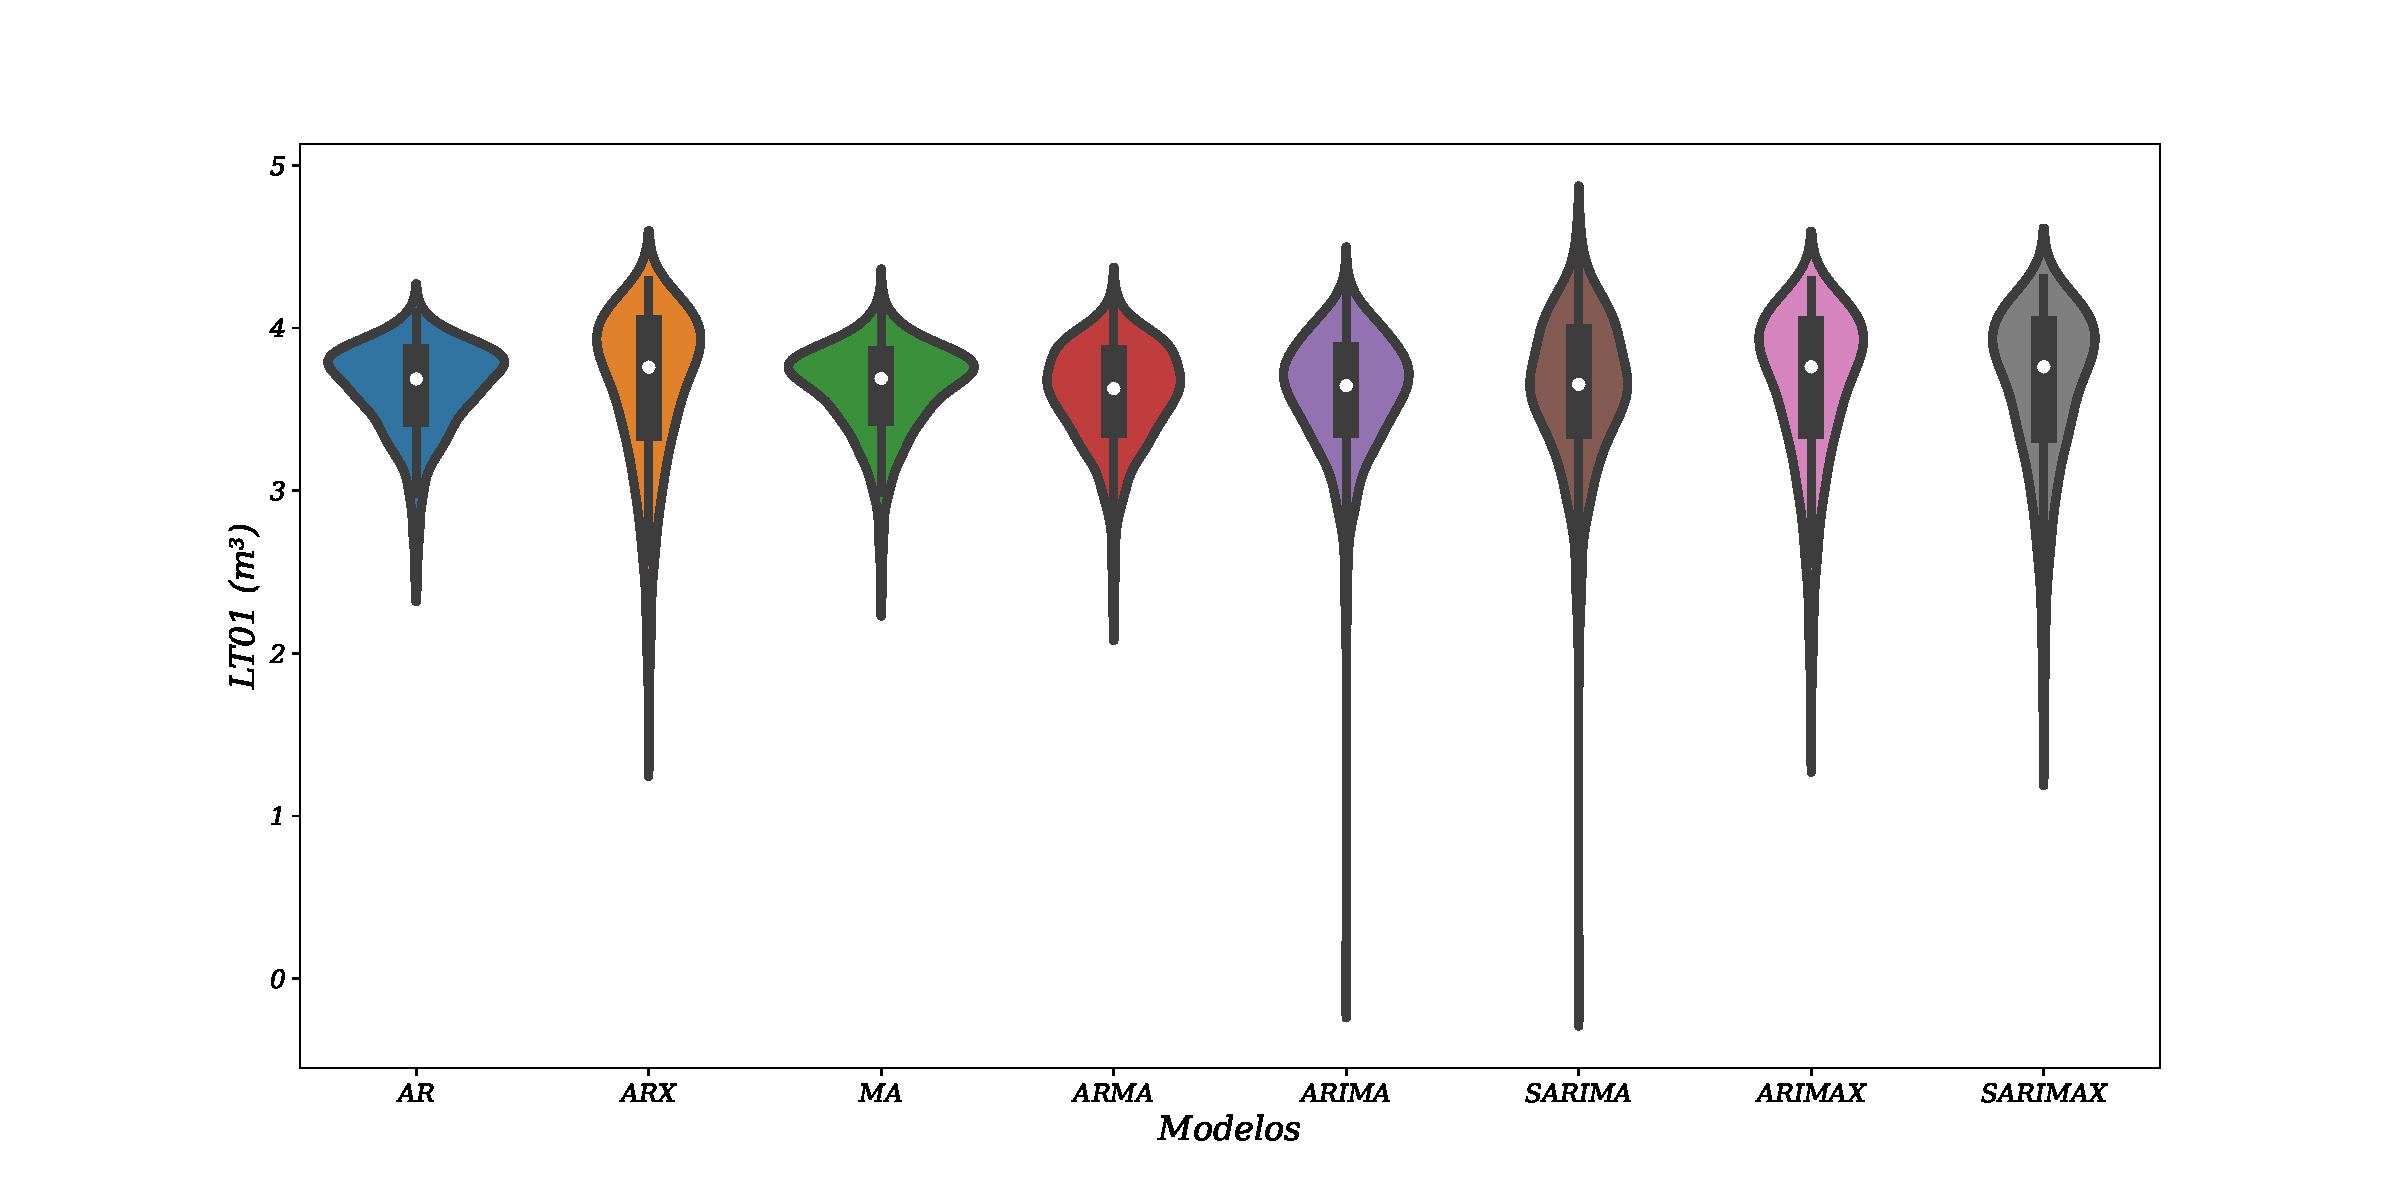
\includegraphics[width=1\linewidth]{Resultados/Figuras/modelos-arima}
	

\end{figure}

Na Figura \ref{fig:violin-lr-xgb-lgbm-rf}, é feita uma comparação entre os modelos de gradiente e regressor. Esses modelos, por serem mais robustos e utilizar técnicas de otimização mais avançadas, mostram-se superiores aos modelos comparados. O modelo XGBoost, em particular, é identificado como superior em relação aos outros modelos na análise.

\begin{figure}[H]
	\centering
	\caption{Comparação de modelos de regressão}\label{fig:violin-lr-xgb-lgbm-rf}
	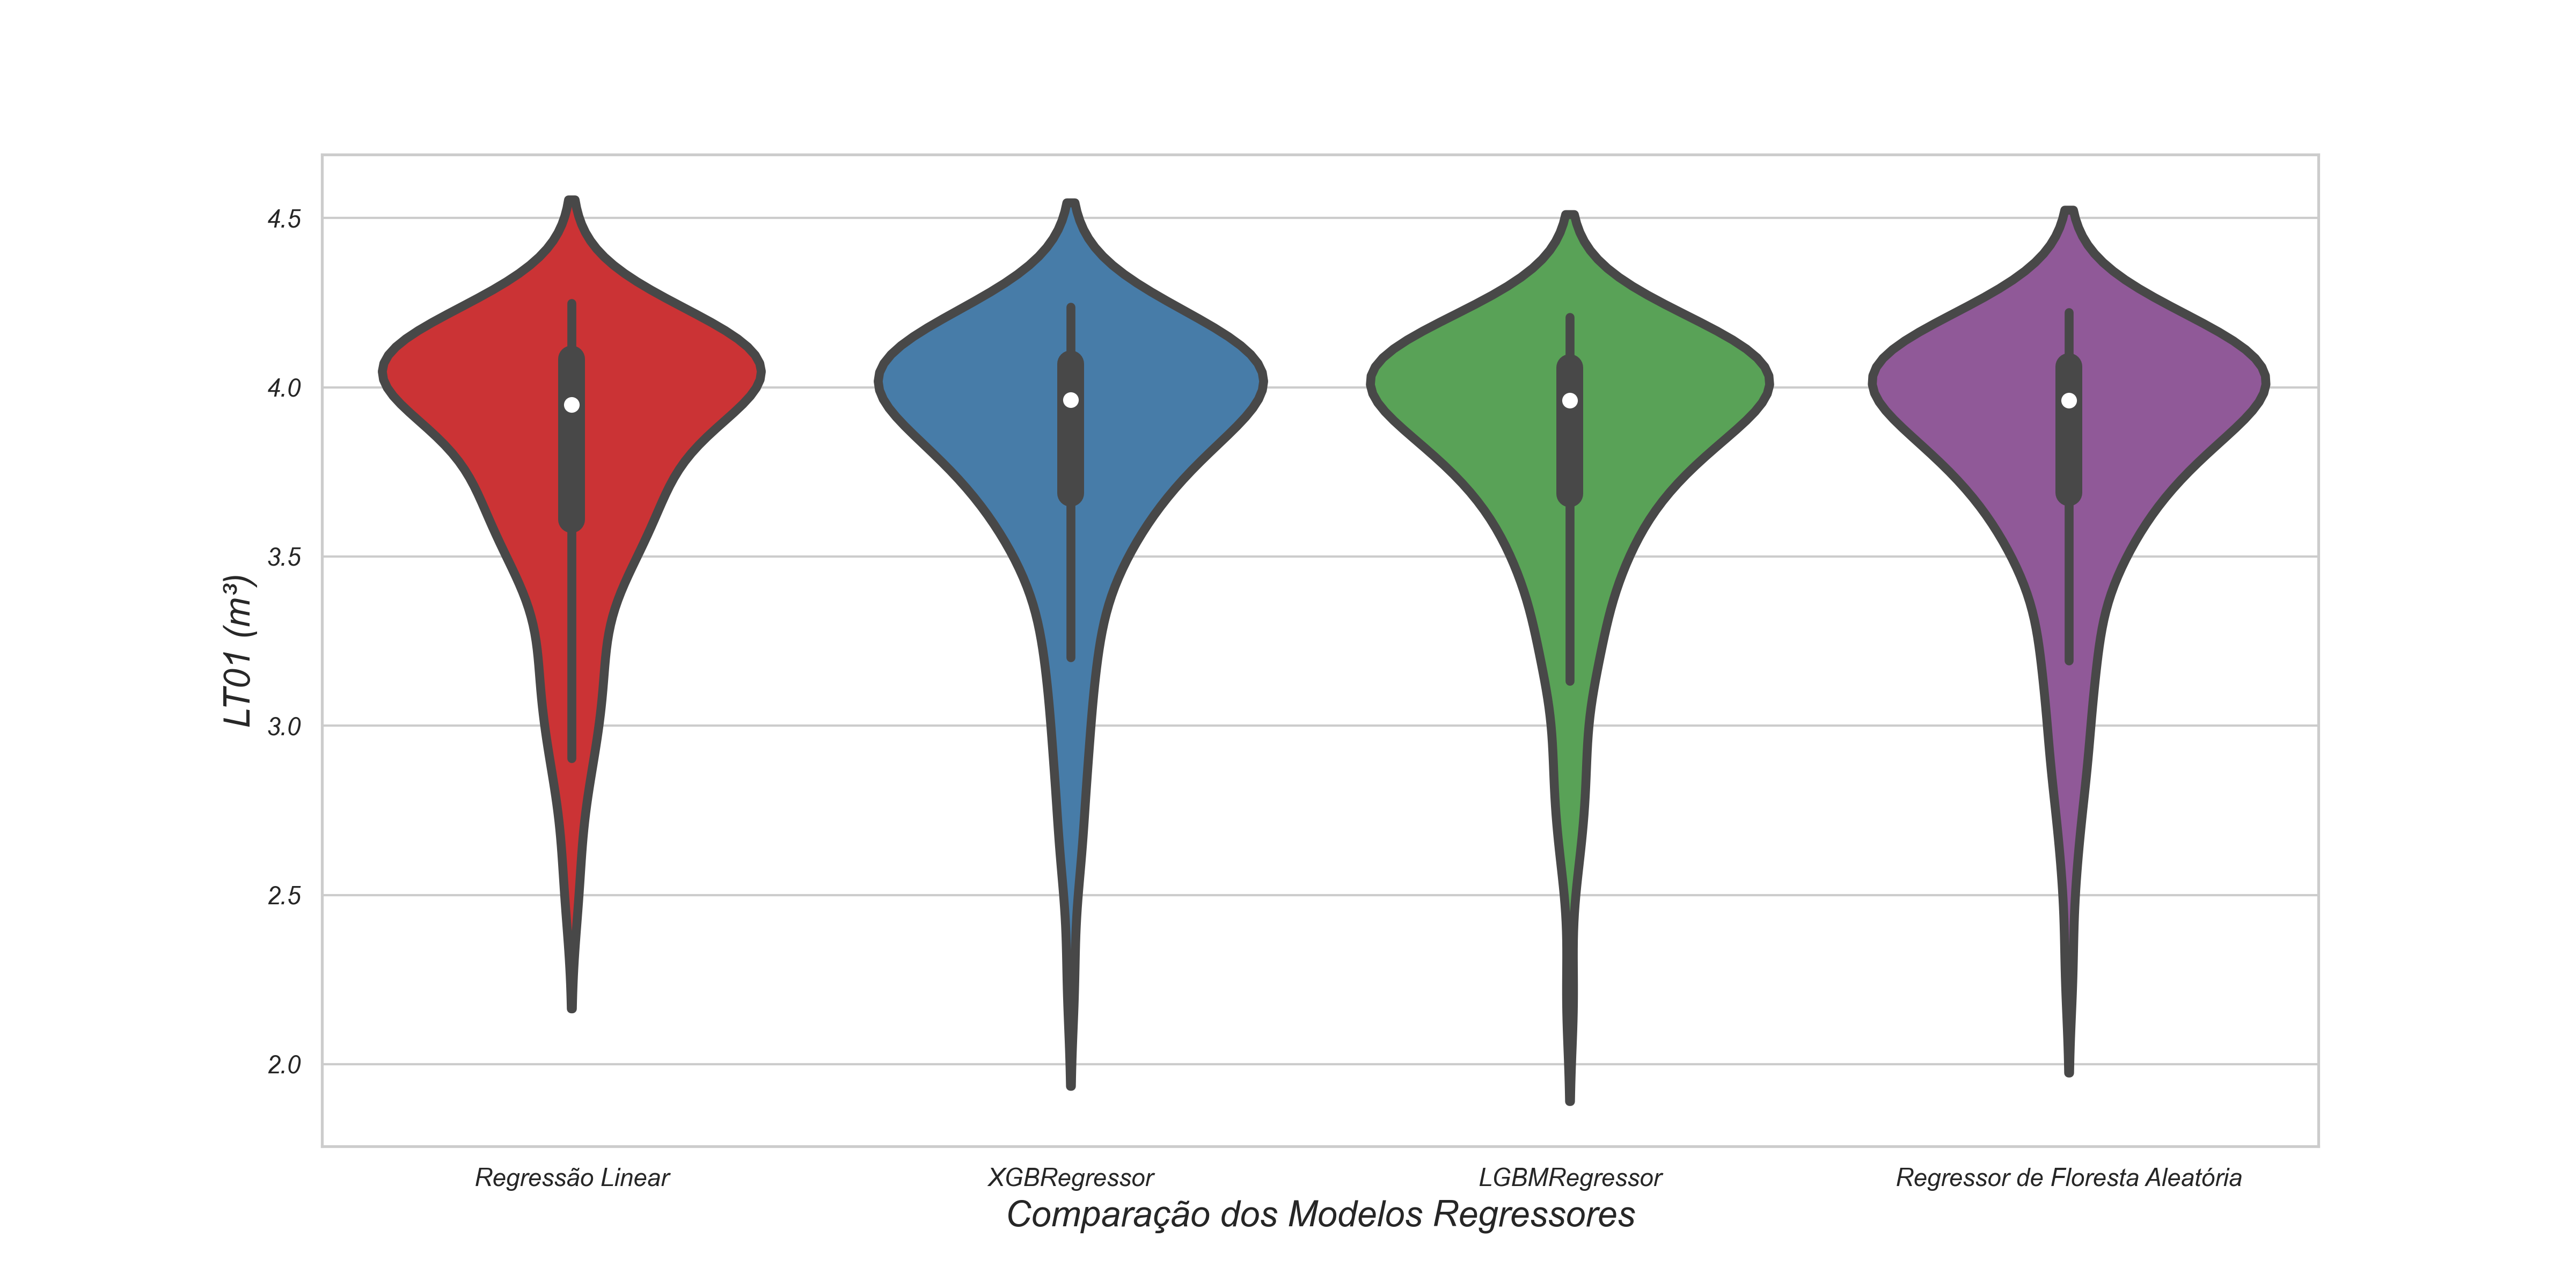
\includegraphics[width=1\linewidth]{Resultados/Figuras/violin-LR-XGB-LGBM-RF}
	
\end{figure}


Na Figura \ref{fig:rrmse_comparar}, nota-se que todos os modelos trabalhados aqui, exceto o modelo LR, foram comparados em relação às métricas de desempenho. Mesmo sendo muito robustos, esses modelos não conseguiram obter um resultado tão bom quanto o RNN.

\begin{figure}[H]
	\centering
	\caption{Análise comparativa dos modelos utilizando gráfico de barras \label{fig:rrmse_comparar} \label{fig:basic_comparar}}
	\begin{subfigure}{1\textwidth}
		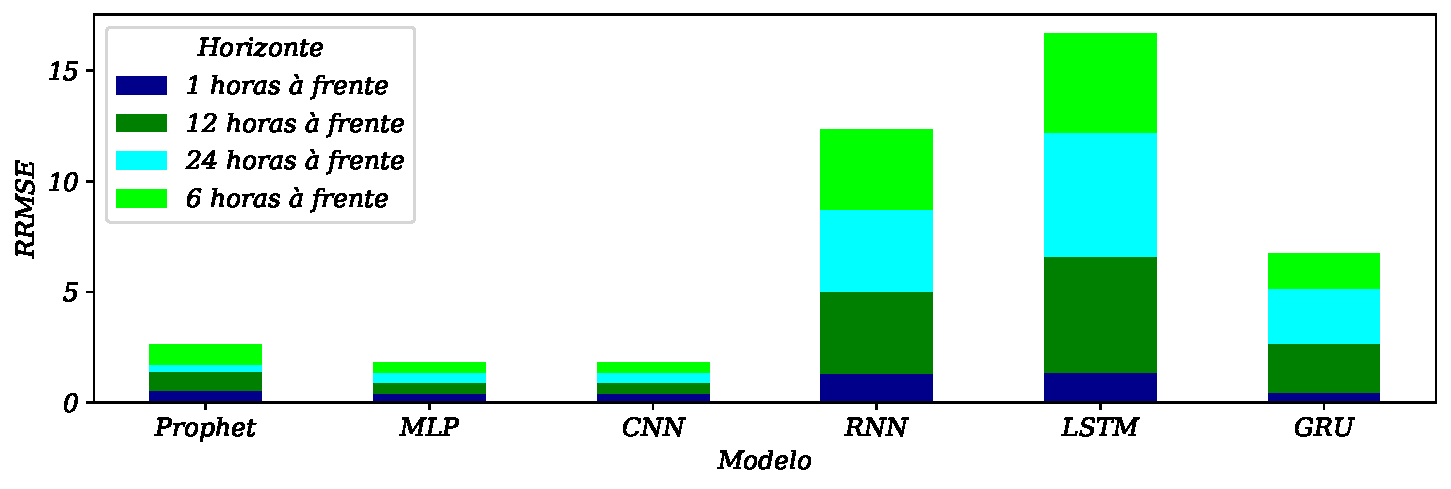
\includegraphics[width=\linewidth]{Resultados/Figuras/rrmse_comparar}
	
		
	\end{subfigure}
	
	\begin{subfigure}{1\textwidth}
		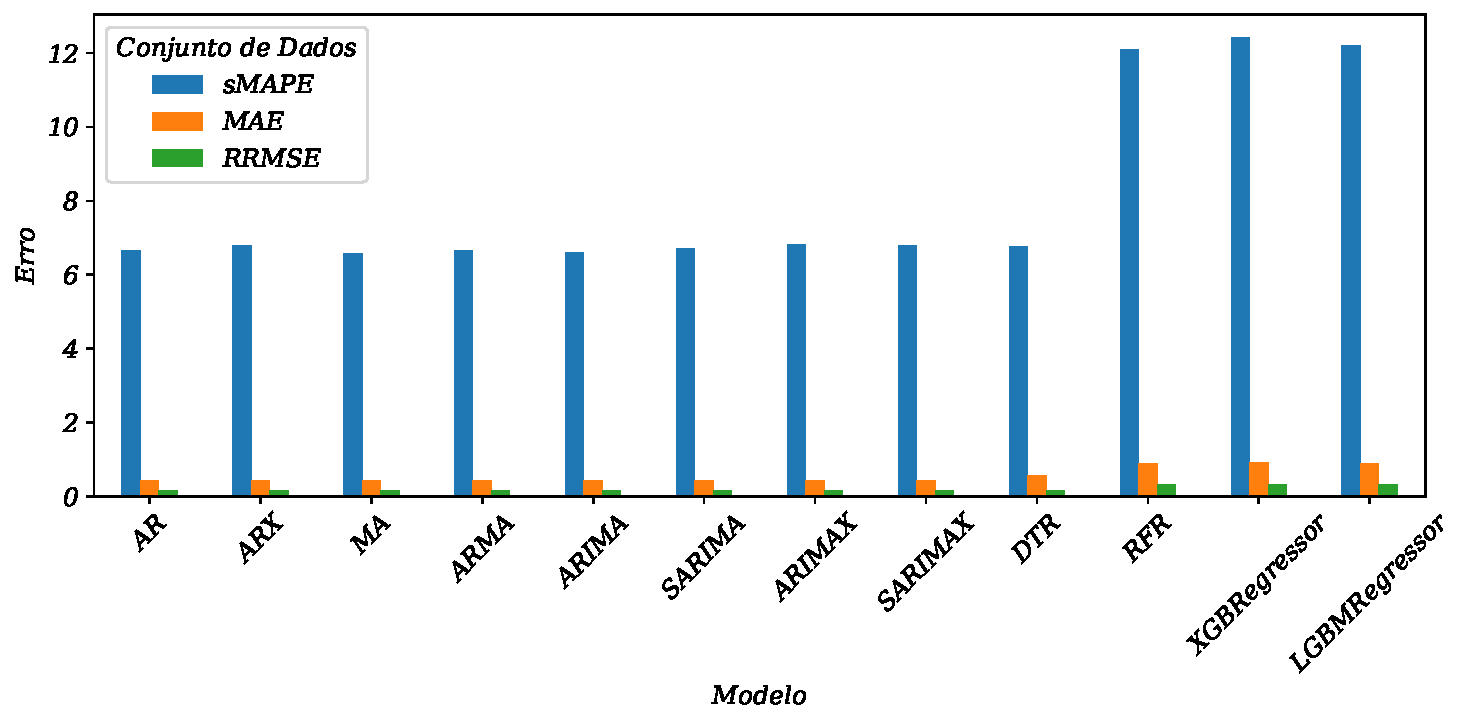
\includegraphics[width=\linewidth]{Resultados/Figuras/basic_comparar}
		
		
	\end{subfigure}
	

\end{figure}

  
 
 

 
  
    

    
